\chapter{Lie theory and Jacobi diagrams}
\label{ch:lie-theory-and-jacobi-diagrams}

The fundamental theorem of Vassiliev invariants states that the bialgebra of Vassiliev invariants can be broken up into nice combinatiorial weight systems. So to understand \(\mathcal{V}\) it suffices to understand \(\mathcal{W}\), or equivalently its dual \(\mathcal{A}\). There is a hint that the structure of \(\mathcal{A}\) may relate to Lie algebras.

\begin{mdframed}
	The hint is that Hopf algebras have a lie algebra as their primitive elements \(\mathcal{P}(H)\). However I clearly am confused here, for the following reason. By the Milnor-Moore theorem, applying this to \(\mathcal{A}\), it should be the symmetric algebra (and therefore the universal enveloping algebra, as it's abelian?) of \(\mathcal{P}(\mathcal{A})\).

	However this clashes with my understanding of the raison d'etre of Hinnich-Vaintrob \cite{cyclic-operads-and-the-algebra-of-chord-diagrams}. According to them, the point of their convoluted construction is to realise \(\mathcal{A}\) as the universal enveloping algebra of some Lie algerba. And a key point is that that's not technically true, hence the need to move to more general tensor categroies.

	Further evidence in \cite{noncommutative-chern-weil-theory-and-the-combinatorics-of-wheeling}: ``The STU relation is a formal analogue of the relation in a Universal Enveloping Algebra which equates a commutator with the corresponding bracket'' (the word formal implying that this isn't literally true).

	Page 141 on \cite{introduction-to-vassiliev-invariants} furthermore says that \cite{cyclic-operads-and-the-algebra-of-chord-diagrams} shows \(\mathcal{A}\) (algebra of Jacobi diagrams on the circle) is isomorphic to the center of the universal enveloping algebra of a Casimir Lie algebra in a certain tensor category. Indeed that's my interpretation of HV, but why do if we already know that \(\mathcal{A}\) is already the center (which in this case equals the whole thing) of \(\mathcal{P}(\mathcal{A})\)?!
\end{mdframed}

% TODO: Try to fix(?) and include the below CDM proof of Milnor-Moore
% \begin{theorem}
% 	The bialgebra \(\mathcal{A}\) is canonically isomorphic to the algebra of polynomials in its primitive elements,
% 	\[\mathcal{A} \cong S(\mathcal{P}(\mathcal{A})),\]
% 	where \(S\) denotes the symmetric algebra.
% \end{theorem}
% \begin{proof}
% 	\begin{mdframed}
% 		The proof in \cite{introduction-to-vassiliev-invariants} is readable, but missing crucial details, and containing a typo. Furthermore I cannot find it anywhere else. If there is time, I want to find out if it works and include it. Perhaps compare to the original source.
% 	\end{mdframed}
% \end{proof}

\section{Jacobi diagrams, AS, STU and IHX}

This side of the story reframes the bialgebra \(\mathcal{A}\) as an isomorphic bialgebra known as the algebra of Jacobi diagrams to illuminate the Lie theory connections.

\begin{definition}
	A \textbf{unitrivalent diagram} is a unitrivalent graph (with loops and multiple edges allowed) with the following additional data:
	\begin{itemize}
		\item each trivalent vertex has a fixed cyclic order of incident edge-connections,
		\item the set of univalent vertices has a fixed cyclic order.
	\end{itemize}
	The vector space of unitrivalent diagrams is denoted \(\mathcal{T}\).
\end{definition}

When drawing unitrivalent diagrams, there are two notation conventions. Firstly, the fixed cyclic order of the univalent edges of is specified by drawing them connected to a circle (the cyclic order is induced by traversing the circle anticlockwise).  Secondly, all the trivalent vertices are taken with the anticlockwise cyclic ordering unless an arrow around that vertex indicates otherwise.

In particular, from the first point, all chord diagrams are unitrivalent diagrams with only univalent vertices (the chord ends). Further examples of unitrivalent diagrams would be
\[
	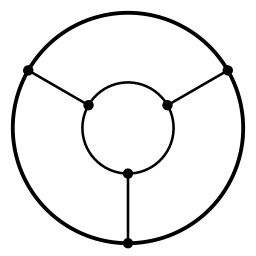
\includegraphics[width=0.13\textwidth, valign=c]{graphics/unitrivalent_diagram_example_1.pdf} \ ,
	\quad
	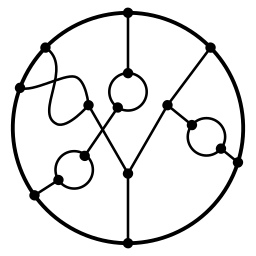
\includegraphics[width=0.13\textwidth, valign=c]{graphics/unitrivalent_diagram_example_2.pdf}
	\in \mathcal{T}.
\]

\begin{definition}
	The \textbf{STU relation} is the relation
		\begin{equation}
			\label{eq:STU}
			\tag{\stu}
			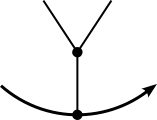
\includegraphics[width=0.10\textwidth, valign=c]{graphics/stu_relation_s.pdf}
			\quad
			=
			\quad
			\includegraphics[width=0.10\textwidth, valign=c]{graphics/stu_relation_t.pdf}
			\quad
			-
			\quad
			\includegraphics[width=0.10\textwidth, valign=c]{graphics/stu_relation_u.pdf}.
		\end{equation}
\end{definition}

As usual, this is not an individual relation but a type of relations, true in any diagrams that are identical except for the subdiagrams being as shown.

Note that the for the chord diagrams inside the algebra of Jacobi diagrams, the \ref{eq:STU} relations imply the \ref{eq:4T} relations, as
	\[
		\adjustbox{valign=c}{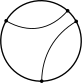
\includegraphics[width=0.115\textwidth]{graphics/four_term_from_stu_north.pdf}}
		\ - \
		\adjustbox{valign=c}{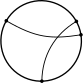
\includegraphics[width=0.115\textwidth]{graphics/four_term_from_stu_south.pdf}}
		\ = \
		\adjustbox{valign=c}{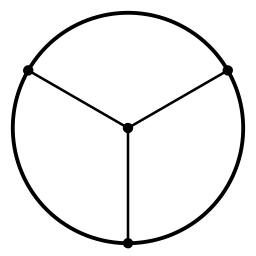
\includegraphics[width=0.12\textwidth]{four_term_jacobi_diagram.pdf}}
		\ = \
		\adjustbox{valign=c}{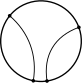
\includegraphics[width=0.115\textwidth]{graphics/four_term_from_stu_west.pdf}}
		\ - \
		\adjustbox{valign=c}{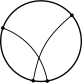
\includegraphics[width=0.115\textwidth]{graphics/four_term_from_stu_east.pdf}}\ .
	\]

\begin{definition}
	The algebra \(\mathcal{J}\) of Jacobi diagrams is the vector space \(\mathcal{T} / \ref{eq:STU}\), with the product \(\connect\) defined the same way as it was for chord diagrams.
\end{definition}

This is well-defined. The proof of Proposition \ref{prop:connected-sum-well-defined} showed that the product \(\connect\) being well-defined on \(\mathcal{A}\) was a consequence of the \ref{eq:4T} relations, which are implied by the \ref{eq:STU} relations. From the \ref{eq:STU} relations, we may deduce the following other relations which hold in \(\mathcal{J}\).

\begin{proposition}
	The following relations are consequences of the \textup{\ref{eq:STU}} relation in \(\mathcal{J}\):
	\begin{enumerate}
		\item The \textbf{AS relation} (antisymmetry relation),
			\begin{equation}
				\label{eq:AS}
				\tag{\as}
				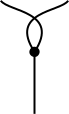
\includegraphics[width=0.05\textwidth, valign=c]{graphics/as_relation_a.pdf}
				\quad
				=
				\quad
				-
				\includegraphics[width=0.05\textwidth, valign=c]{graphics/as_relation_s.pdf}.
			\end{equation}
		\item The \textbf{IHX relation},
			\begin{equation}
				\label{eq:IHX}
				\tag{\ihx}
				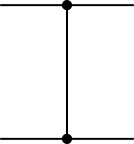
\includegraphics[width=0.10\textwidth, valign=c]{graphics/ihx_relation_i.pdf}
				\quad
				=
				\quad
				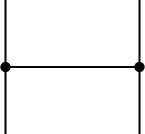
\includegraphics[width=0.10\textwidth, valign=c]{graphics/ihx_relation_h.pdf}
				\quad
				-
				\quad
				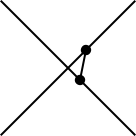
\includegraphics[width=0.10\textwidth, valign=c]{graphics/ihx_relation_x.pdf}.
			\end{equation}
	\end{enumerate}
\end{proposition}

\begin{proof}
	% TODO: Maybe put some images here.
	\begin{enumerate}
		\item
			Take two diagrams which differ only by \ref{eq:AS} at one (trivalent) vertex. If the vertex at which the \ref{eq:AS} relation resides is adjacent to a univalent vertex (i.e. touches the outer circle), then this is immediate from applying \ref{eq:STU} to both diagrams at that vertex.

			If the vertex is not immediately adjacent to a univalent vertex, then it is some \(d\) vertices `in the way'. By applying \ref{eq:STU} to those vertices yields a sum of \(2^{d}\) diagrams, all identical except for differing by \ref{eq:AS}, now on a vertex adjacent to a univalent vertex.

		\item
			A similar argument applies. If one of the two vertices of the \ref{eq:IHX} is adjacent to the circle, then the result is a direct consequence of an \ref{eq:STU} on each of the vertices. Otherwise, some \ref{eq:STU}s may be required first.
\end{enumerate}
\end{proof}

Looking at the relations \ref{eq:STU}, \ref{eq:AS} and \ref{eq:IHX}, the first solid evidence of Lie-theoretic structure in this story emerges. Explicit connections will be the subject of the next subsection, but for now notice that interpreting the trivalent vertex in \ref{eq:STU} (which has two `input' edges above and one `output' edge below) as a bracket, this bears resembelance to the relation that defines the universal enveloping algebra of a Lie algebra \([x, y] = xy - yx\). Similarly, \ref{eq:AS} looks like the antisymmetry property of the bracket \([x, y] = -[y, x]\). For \ref{eq:IHX} perhaps the relation isn't quite so obvious until the diagrams are rearranged into the form
\begin{equation*}
	\tag{\ihx}
	\includegraphics[width=0.10\textwidth, valign=c]{graphics/ihx_jacobi_form_i.pdf}
	\quad
	=
	\quad
	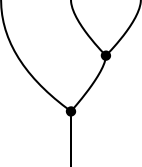
\includegraphics[width=0.10\textwidth, valign=c]{graphics/ihx_jacobi_form_h.pdf}
	\quad
	+
	\quad
	\includegraphics[width=0.10\textwidth, valign=c]{graphics/ihx_jacobi_form_x.pdf},
\end{equation*}
(here also one application of \ref{eq:AS} was used) whereby the \ref{eq:IHX} looks like the Jacobi identity, in the form \([[x, y], z] = [x, [y, z]] + [y, [x, z]]\).

\begin{lemma}[Generalised \ref{eq:IHX}]
	The following holds in \(\mathcal{J}\) for any subgraph consisting of trivalent vertices that can be inserted into the grey box.
	\[
		\sum_{i = 0}^{m}\
		\def\svgscale{0.3}
		\raisebox{-34pt}{\input{graphics/generalised_ihx_left.pdf_tex}}
		\quad
		=
		\quad
		\sum_{i = 0}^{n}\
		\def\svgscale{0.3}
		\raisebox{-34pt}{\input{graphics/generalised_ihx_right.pdf_tex}}
	\]
\end{lemma}

The result is standard, see Chapter 5.2 of \cite{introduction-to-vassiliev-invariants} for a proof.
% TODO: Maybe I want to prove this.

% TODO: The change of basis assumption here is a liiitle sus.
We have already spoiled the surprise that in the end, \(\mathcal{A}\) and \(\mathcal{J}\) will be isomorphic as bialgebras. In fact, as algebras, this is clearly true so far, as \(\mathcal{J}\) is just a change of basis from \(\mathcal{A}\). Since \(\mathcal{A}\) spans \(\mathcal{J}\), we can attempt to lift the coproduct from \(\mathcal{A}\) directly onto \(\mathcal{J}\).

\begin{proposition}
	The coproduct \(\Delta\) on \(J \in \mathcal{J}\) defined by taking a Jacobi diagram, representing it as a chord diagram via \textup{\ref{eq:STU}}, taking the coproduct in \(\mathcal{A}\), then interpreting the result as a Jacobi diagram via the inclusion of \(\mathcal{A}\) into \(\mathcal{J}\), is also given by the following formula.

	\[\Delta(J) = \sum_{C \subset S} J_{C} \otimes J_{\overline{C}},\]
	where \(S\) is the set of connected components of \(J\), and \(\overline{C} = S \smallsetminus C\).
\end{proposition}

\begin{proof}
	Note that this has the same symbolic form as the coproduct in \(\mathcal{A}\) given in Definition~\ref{def:coproduct-in-chord-diagrams}, but with chords replaced by connected components of Jacobi diagrams. However, when working in \(\mathcal{A} \subset \mathcal{J}\), there are only univalent vertices, so the connected components are exactly the chords. Since \(\mathcal{A}\) forms a basis for \(\mathcal{J}\), and the formula is linear, it extends to all of \(\mathcal{J}\).
\end{proof}

\begin{corollary}
	The primitive elements \(\mathcal{P}(\mathcal{A})\) are the connected Jacobi diagrams.
\end{corollary}

\begin{corollary}
	The bialgebras \(\mathcal{A}\) and \(\mathcal{J}\) are isomorphic.
\end{corollary}

\begin{warning}
	Justified by this isomorphism, we write \(\mathcal{J} = \mathcal{A}\), and \(\mathcal{A}\) is the preferred choice of notation for both chord diagrams and Jacobi diagrams.
\end{warning}

\section{Lie algebra weight systems}
Similar diagrammatic relations to \ref{eq:STU}, \ref{eq:AS} and \ref{eq:IHX} satisfied by \(\mathcal{A}\) are appear also in the context of a graphical notation for multilinear maps, a fact which we may exploit to probe \(\mathcal{A}\). Before seeing how, let us review this graphical notation following \cite{wheeling-a-diagrammatic-analogue-of-the-duflo-isomorphism, on-the-rozansky-witten-weight-systems}.

\begin{remark}
	This diagrammatic calculus is well-known but it goes by many names: Penrose calculus, tensor calculus, diagrammatic calculus for tensors, etc. A rarely seen but accurate name is `tensor diagrammar'.
\end{remark}

A tensor, i.e. a multilinear map takes as its input a tensor product of \(m\) various vector spaces, and has as output a a tensor product of \(n\) various vector spaces. Such a map can be represented as a vertex with \(m + n\) unbound edges; \(m\) decorated by the corresponding vector spaces with incoming arrows, and \(n\) decordated by the corresponding vector spaces again with outgoing arrows.

For example, the bracket in a Lie algebra \(\mathfrak{g}\) is a map \([\cdot,\cdot] \in \mathfrak{g}^{\ast} \otimes \mathfrak{g}^{\ast} \otimes \mathfrak{g}\), expressed as
\[\text{Lie bracket vertex}\]

Such a notation is useful because composition of tensors can be expressed graphically by connecting outgoing and incoming legs with the same decoration. Relations can therefore be expressed graphically, for example, the antisymmetry of the bracket \([x, y] = -[y, x]\) becomes
\[\text{\ref{eq:AS}}\]
the Jacobi relation \([[x, y], z] + [[y, z], x] + [[z, x], y] = 0\) becomes
\[...\ .\]

A representation \(\rho\) of a Lie algebra is a vertex of type
\[...\]
and the equation that \(\rho\) be a lie algebra representation is the diagrammatic statement
\[...\ .\]

If \(\mathfrak{g}\) is a metric Lie algebra (i.e. it has an invariant, nondegenerate bilinear form) then we have an additional vertex with both input edges labelled \(\mathfrak{g}\). Since it's nondegenerate, it can be inverted to achieve a vertex with both output edges labelled \(\mathfrak{g}^{\ast}\). This allows the composition of the bracket vertices with signature \(\mathfrak{g}^{\ast} \otimes \mathfrak{g}^{\ast} \otimes \mathfrak{g}\) into vertices with signature \(\mathfrak{g} \otimes \mathfrak{g} \otimes \mathfrak{g}\), or vice \(\mathfrak{g}^{\ast} \otimes \mathfrak{g}^{\ast} \otimes \mathfrak{g}^{\ast}\). Since they are invertible, they can be inserted anywhere without losing information.

Moreover, the invariance of the form can be written as \(\langle [x, y], z \rangle = \langle [z, x], y \rangle\) which graphically can be represented as cyclic invariance of the composition of these vertices
\[... = ... = ... \ .\]
This justifies drawing only vertices of type
\[composition\]
which are equal to any of the above.

The famous construction of Bar-Natan \cite{on-the-vassiliev-knot-invariants} uses this diagrammatic calculus to take metric Lie algebras and produce weight systems.

% TODO: According to Chmutov-Duzhin-Mostovoy, p164, the weight system is only multiplicative if the representation is irreducible. Question for Zsuzsi: does this mean we only get a quotient of A if we put in an irreducible representation?
\begin{theorem}
	The construction below which takes a lie algebra \(\mathfrak{g}\) produces a well-defined weight system \(W_{\mathfrak{g}}\) valued in \(\mathcal{U}(\mathfrak{g})\).
	% TODO: Should this be Q?
	Furthermore if a representation, \(\rho\) of \(\mathfrak{g}\) is given, then a \(\mathbb{C}\)-valued weight system is produced.
\end{theorem}

\begin{construction}
	Given a Lie algebra \(\mathfrak{g}\), the vertex \(m\) with signature \(\mathfrak{g} \otimes \mathfrak{g} \otimes \mathfrak{g}\) is associated to a genuine element of the tensor algebra \(T_{\mathfrak{g}}(m) \in \mathfrak{g}^{\otimes 3}\). For each trivalent vertex of the Jacobi diagram \(J \in \mathcal{A}\), take \(T_{\mathfrak{g}}(m)\), and take all of their tensor products, in arbitrary order. There being \(v\) trivalent vertices, this lies in \(\mathfrak{g}^{\otimes 3v}\).

	For each edge between the trivalent vertices in the Jacobi diagram, contract the corresponding variables in \(\mathfrak{g}^{\otimes 3 v}\). The result lies in \(\mathfrak{g}^{\otimes 3v - 2e}\) where \(e\) is the number of edges between trivalent vertices.

	The number of univalent vertices matches the number of remaining uncontracted trivalent vertices, \(u = 3v - 2e\). In-particular the edges between univalent and trivalent vertices, along with the cyclic order on univalent vertices determines a cyclic order on the remaining trivalent vertices. So, a cyclic order on the factors of \(\mathfrak{g}^{\otimes 3v - 2e} = \mathfrak{g}^{\otimes u}\). Permute the factors into an order which respects the induced cyclic order (there are many --- choose one). Projecting from the tensor algebra of \(\mathfrak{g}\) into its universal enveloping algebra, we obtain an element \(W_{\mathfrak{g}}(J) \in \mathcal{U}(\mathfrak{g})\).

	A representation \(\rho: \mathfrak{g} \to \operatorname{Hom}(V)\) of \(\mathfrak{g}\) extends uniquely to a representation \(\rho: \mathcal{U}(\mathfrak{g}) \to \operatorname{Hom}(V)\) of \(\mathcal{U}(\mathfrak{g})\). Use this representation to take the trace of \(W_{\mathfrak{g}}(J)\). The result is an element of the ground field \(W_{\mathfrak{g}, \rho}(J) = \operatorname{tr}(\rho(T_{\mathfrak{g}}(J))) \in \mathbb{C}\).
\end{construction}

\begin{warning}
	When constructing \(T_{\mathfrak{g}}(m)\), the tensor factors in the tensor corresponding to the bracket need to have the unusual cyclic order \((y, x, [x, y]_{\mathfrak{g}})\). This is because its projection into \(\mathcal{U}(\mathfrak{g})\) should obey \ref{eq:STU}, and this is the cyclic order of the trivalent vertex in \ref{eq:STU}.
\end{warning}

Hence, we have the functions \(W_{\mathfrak{g}}: \mathcal{A} \to \mathcal{U}(\mathfrak{g})\) and \(W_{\mathfrak{g}, \rho}: \mathcal{A} \to \mathbb{C}\) which we claim are weight systems.

\begin{proof}

	The Penrose diagrams constructed out of the vertices of the type listed above are well-defined as planar graphs \cite[Proposition 3.1.1]{vassiliev-knot-invariants-and-lie-s-algebras}. Thus since the tensor is constructed only from contractions of the above vertices, it is determined by the information of which components are contracted, and their order in the final tensor. This information is encoded by a uni-trivalent graph with an ordering on its univalent vertices.

	To prove that the map \(W_{\mathfrak{g}}: \mathcal{A} \to \mathcal{U}(\mathfrak{g})\) is well-defined it suffices to show that the Penrose diagrams obey the \(\ref{eq:STU}\) relations when interpreted as elements of \(\mathcal{U}(\mathfrak{g})\). If two chord diagrams differ by \ref{eq:STU}, on some univalent vertices associated with adjacent tensor factors \(y\) and \(x\), the construction gives
	\[\cdots \otimes [x, y]_{\mathfrak{g}} \otimes \cdots \qquad \text{and} \qquad (\cdots \otimes x \otimes y \otimes \cdots) - (\cdots \otimes y \otimes x \otimes \cdots),\]
	but this equality is exactly the quotient in the \(\mathcal{U}(\mathfrak{g})\).

	Indeed \ref{eq:AS} and \ref{eq:IHX} follow from \ref{eq:STU} but they are also easy to see directly. \(\ref{eq:AS}\) follows from the skew-symmetry of the vertex \(m\), being built out of the bracket, and \(\ref{eq:IHX}\) follows from the Jacobi identity in \(\mathfrak{g}\).

	Finally, a Jacobi diagram's univalent vertices only have a cyclic order. But in the construction a true order respecting that cyclic order was chosen. We should show that any order respecting the cyclic order leads to the same result. It suffices to show that the tensor is cyclically symmetric. Indeed, a stronger statement is true: anything satisfying the \ref{eq:STU} relation is cyclically symmetric. Since it is stronger, let us prove it instead for \(\mathcal{A}\).

	It is equivalent to prove that any Jacobi diagram on a long line is cyclically symmetric. Examine the operation of taking the univalent vertex (which we will here call legs) in the first position and moving it to the last position, reducing by one the positions of all other legs. This generates the cyclic group on the number of univalent vertices, so it is enough to show this operation preserves the Jacobi diagram. The \ref{eq:STU} relation gives the cost of commuting the first leg past the \(i\)th leg: the same diagram with the first leg attached to the \(i\)th leg. Thus cost commuting the first leg to the very last place is the sum over the other legs of attaching it to those legs. We will show that this cost is zero.

	We split this sum by the connected components of the \(i\)th leg. On components that don't contain the first leg, this is the sum, over legs, of the same diagram, with the first leg attached to the \(i\)th leg. This vanishes by the generalised \ref{eq:IHX}. On the component that contains the first leg, this sum is also killed by generalised \ref{eq:IHX}, as it produces a diagram with a loop at the top.
\end{proof}

\begin{remark}
	% TODO: Call the Penrose diagrams something consistent throughout.
	We showed in the proof above that the Penrose diagrams with given vertices obey \ref{eq:STU}. Such an object is starting to look a lot like a Jacobi diagram. We showed that these objects satisfy the \ref{eq:STU} relations, but it's still possible they satisfy more relations than Jacobi diagrams, a statement which we will formalise in Section \ref{sec:non-lie-algebraic-weight-systems}.
\end{remark}

\begin{mdframed}
	Confirm: This obeys all the relations of \(\mathcal{A}\), and more. Does this make it a quotient of \(\mathcal{A}\)?
\end{mdframed}

Let's look at a specific weight system for the Lie algebra \(\mathfrak{sl}_{2}\) \cite{on-the-vassiliev-knot-invariants, remarks-on-the-vassiliev-knot-invariants-coming-from-sl2}.
\begin{example}[Weight system for \({\mathfrak{sl}_{2}}\)]
	We choose as our Lie algebra \(\mathfrak{sl}_{2}\), generated by \(h\), \(e\) and \(f\) with commutators
	\[[h, e] = 2e, \quad [h, f] = -2f, \quad [e, f] = h.\]
	The unique invariant form up to scalar multiple is
	\[\langle h, h \rangle = 1, \quad \langle e, f \rangle = \frac{1}{2}, \quad \langle f, e \rangle = \frac{1}{2},\]
	and all other inner products are zero.

	In \cite{remarks-on-the-vassiliev-knot-invariants-coming-from-sl2}, the following skein relation is derived:
	\[
		W_{\mathfrak{sl}_{2}}
		\left(
			\includegraphics[width=0.115\textwidth, valign=c]{graphics/sl2_skein_relation_h.pdf}
		\right)
		=
		4 W_{\mathfrak{sl}_{2}}
		\left(
			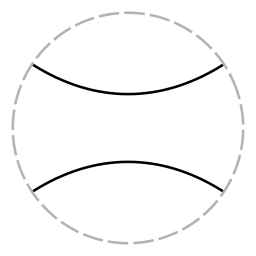
\includegraphics[width=0.115\textwidth, valign=c]{graphics/sl2_skein_relation_uu.pdf}
		\right)
		-
		4 W_{\mathfrak{sl}_{2}}
		\left(
			\includegraphics[width=0.115\textwidth, valign=c]{graphics/sl2_skein_relation_x.pdf}
		\right)
	\]

	\begin{proof}
		Associated to the Penrose diagram for each side of the above equation (it is not advisable to compute by hand) we find the tensors
		\begin{align*}
			{}- 8 h\otimes e\otimes h\otimes f && {}+ 8 & h\otimes e\otimes f\otimes h & {}- \phantom{1}8  & h\otimes f\otimes h\otimes e & {}+ \phantom{1}8  & h\otimes f\otimes e\otimes h \\
			{}+ 8 e\otimes h\otimes h\otimes f && {}- 8 & e\otimes h\otimes f\otimes h & {}+            16 & e\otimes f\otimes e\otimes f & {}-            16 & e\otimes f\otimes f\otimes e \\
			{}+ 8 f\otimes h\otimes h\otimes e && {}- 8 & f\otimes h\otimes e\otimes h & {}-            16 & f\otimes e\otimes e\otimes f & {}+            16 & f\otimes e\otimes f\otimes e
		\end{align*}
		and
		\begin{align*}
			{}+ 8 h\otimes h\otimes e\otimes f && {}+ \phantom{1}8  & h\otimes h\otimes f\otimes e & {}- \phantom{1}8  & h\otimes e\otimes h\otimes f & {}- \phantom{1}8  & h\otimes f\otimes h\otimes e \\
			{}- 8 e\otimes h\otimes f\otimes h && {}- 16 & e\otimes e\otimes f\otimes f & {}+ \phantom{1}8  & e\otimes f\otimes h\otimes h & {}+ 16 & e\otimes f\otimes e\otimes f \\
			{}- 8 f\otimes h\otimes e\otimes h && {}+ \phantom{1}8  & f\otimes e\otimes h\otimes h & {}+ 16 & f\otimes e\otimes f\otimes e & {}- 16 & f\otimes f\otimes e\otimes e.
		\end{align*}
		Projecting into \(\mathcal{U}(\mathfrak{g})\) and using one's favourite CAS to express both expressions in the Poincare-Birkhoff-Witt basis, we find both equal to
		\[64 e \otimes f + 16 h \otimes h - 32 h.\]
	\end{proof}
\end{example}

\begin{mdframed}
	literature summary of tables of dimensions from metric Lie algebras.
\end{mdframed}

\section{Non-Lie algebraic weight systems}
\label{sec:non-lie-algebraic-weight-systems}

\begin{mdframed}
	The IHX, STU, AS is slightly more than just the jacobi; the tensor algebra isomorphism can be other than the identity (e.g. superalgebras).
\end{mdframed}

\begin{mdframed}
	gl(1, 1) as an example
\end{mdframed}

\begin{mdframed}
	Results of Vogel and calculations of Lieberum.
\end{mdframed}

\section{Jacobi diagrams as a universal enveloping algebra}
